%%%NOTE: for help with latex symbols look here http://mirror.unl.edu/ctan/info/symbols/comprehensive/symbols-a4.pdf.
\documentclass[12pt]{article}
\usepackage{color}
\usepackage{cite}
\usepackage{geometry}                % See geometry.pdf to learn the layout options. There are lots.
%\usepackage{pdflscape}        %single page landscape
                                %mode \begin{landscape} \end{landscape}
\geometry{letterpaper}                   % ... or a4paper or a5paper or ... 
%\usepackage[parfill]{parskip}    % Activate to begin paragraphs with an empty line rather than an indent
\usepackage{multicol} % \begin{multicols}{number of columns} \end{multicols}
\usepackage{graphicx}
\usepackage{amssymb}
\usepackage{Sweave}
\newcommand{\etal}{\textit{et al.}}
\newcommand{\R }{\textbf{R}}
\usepackage[cp1252]{inputenc} 
\inputencoding{cp1252}
\usepackage{hyperref}  %\hyperref[label_name]{''link text''}
                       %\hyperlink{label}{anchor caption}
                       %\hypertarget{label}{link caption}
\linespread{1.5}

\title{ComGenR: Community Genetics Analyses in \R}
\author{M.K. Lau}
%\date{}                                           % Activate to display a given date or no date

\begin{document}
\maketitle

Community Genetics is a field that works at the interface between
ecological genetics and community ecology. Being inherently
multi-disciplinary, the analytics involved have developed in separate
fields. \textit{ComGenR} is intended to synthesize these analytical
techniques and facilitate new analytically and computationally driven
research tools. Here, we present an introduction to the package,
broken into five main sections:

\setcounter{tocdepth}{3}  %%activate to number sections
\tableofcontents  


\section{Community Genetics Data}

Two primary aims of Community Genetics (CG) research are to test and
quantify how genetic variation influences the distribution of species
in a community \cite{whitham2006}. These studies have typically
examined the composition of a community of organisms associated with
individuals of a focal species (e.g. \cite{keith2010}
\cite{shuster2006} \cite{bailey2006}), which is most often a
foundation species \cite{ellison2005}. Thus, CG datasets tend to be in
a community ecology form with sets individuals with multivariate
observations of the abundances of associated species and
phenotypic and/or genetic information. These data are most often
compiled and curated using spreadsheets (e.g. Microsoft Excel). 

When working in \R, these data are most easily managed and imported if
they are in a standardized column format, where the first column is a
set of labels for each column. For more detailed introduction to \R, a quick
google search for ``ecological analysis in R'' will guide you to many
resources, including my introductory course
\href{http://perceval.bio.nau.edu/downloads/igert/IntroR-Course_Notes/R-Course.pdf}{here}.

%Species abundances
%Genetic information
%Brief mention of other packages
%Importing data

In order allow for users to extend \R's functionality, functions are
grouped together into ``packages'' by programmers. This allows for \R to
be reduced to a core set of software that can be added to by obtaining
and loading these other packages. At current count (March 2012), there
are over 4000 packages contributed by the \R software community. This
means, however, that any package that is not contained in the core \R
distribution must be downloaded initially and each time \R is opened
the package must be ``libraried'' (i.e. loaded into the working memory).

Here is the easiest way to do this:

\begin{Schunk}
\begin{Sinput}
>   install.packages('ComGenR')
> 
\end{Sinput}
\end{Schunk}

\begin{Schunk}
\begin{Sinput}
> library(ComGenR)
> 
\end{Sinput}
\end{Schunk}

Once you have run \texttt{install.packages}, you'll only need to run
\texttt{library} when you open up \R. 

You can get some quick information on the package and any function by
using the question mark symbol:

\begin{Schunk}
\begin{Sinput}
> ?ComGenR
> 
\end{Sinput}
\end{Schunk}

Here, we will use an example dataset of
a set of trees with genotypic and community data called
\textit{cg\_data.csv}. Let's load the data and take a quick look at
it's properties:


\begin{Schunk}
\begin{Sinput}
> the.data <- read.csv('cg_data.csv')
> 
\end{Sinput}
\end{Schunk}

\begin{Schunk}
\begin{Sinput}
> colnames(the.data)
\end{Sinput}
\begin{Soutput}
 [1] "tree.id" "geno"    "pheno"   "S1"      "S2"      "S3"      "S4"     
 [8] "S5"      "S6"      "S7"      "S8"      "S9"      "S10"     "S11"    
[15] "S12"     "S13"     "S14"     "S15"     "S16"     "S17"     "S18"    
[22] "S19"     "S20"     "S21"     "S22"     "S23"     "S24"     "S25"    
\end{Soutput}
\begin{Sinput}
> 
\end{Sinput}
\end{Schunk}

\begin{Schunk}
\begin{Sinput}
> summary(the.data)
\end{Sinput}
\begin{Soutput}
    tree.id        geno          pheno             S1           
 tree_1 : 1   Min.   : 1.0   Min.   :11.00   Min.   :  0.00001  
 tree_10: 1   1st Qu.: 3.0   1st Qu.:13.75   1st Qu.:  0.00001  
 tree_11: 1   Median : 5.5   Median :15.62   Median : 13.68308  
 tree_12: 1   Mean   : 5.5   Mean   :15.62   Mean   : 34.01201  
 tree_13: 1   3rd Qu.: 8.0   3rd Qu.:17.50   3rd Qu.: 69.16127  
 tree_14: 1   Max.   :10.0   Max.   :21.00   Max.   :114.37323  
 (Other):44                                                     
       S2                 S3                  S4                  S5        
 Min.   :  0.4626   Min.   :  0.00001   Min.   :  0.00001   Min.   : 14.45  
 1st Qu.: 67.2984   1st Qu.:  0.00001   1st Qu.: 70.77429   1st Qu.: 71.11  
 Median : 81.8078   Median : 20.49474   Median : 90.58988   Median : 85.99  
 Mean   : 82.8257   Mean   : 35.23070   Mean   : 84.21616   Mean   : 84.70  
 3rd Qu.:107.5850   3rd Qu.: 64.73125   3rd Qu.:102.75975   3rd Qu.:105.23  
 Max.   :129.1476   Max.   :110.66000   Max.   :125.48962   Max.   :123.51  
                                                                            
       S6                 S7                  S8                S9           
 Min.   :  0.3502   Min.   :  0.00001   Min.   :  9.496   Min.   :  0.00001  
 1st Qu.: 69.3803   1st Qu.:  0.00001   1st Qu.: 72.335   1st Qu.: 44.23739  
 Median : 91.2332   Median : 26.69620   Median : 92.194   Median : 78.05749  
 Mean   : 85.4561   Mean   : 39.75816   Mean   : 88.753   Mean   : 70.28158  
 3rd Qu.:105.5072   3rd Qu.: 79.23763   3rd Qu.:106.059   3rd Qu.: 99.39094  
 Max.   :126.0525   Max.   :121.37132   Max.   :128.524   Max.   :126.78093  
                                                                             
      S10                 S11                 S12                 S13        
 Min.   :  0.00001   Min.   :  0.00001   Min.   :  0.00001   Min.   : 19.57  
 1st Qu.: 42.00070   1st Qu.:  0.00001   1st Qu.: 43.93994   1st Qu.: 67.95  
 Median : 80.82798   Median :  0.00001   Median : 79.87761   Median : 88.40  
 Mean   : 71.06607   Mean   : 24.74326   Mean   : 75.58593   Mean   : 84.82  
 3rd Qu.: 99.64315   3rd Qu.: 37.08868   3rd Qu.:104.02991   3rd Qu.:107.96  
 Max.   :115.04995   Max.   :112.32940   Max.   :126.79579   Max.   :125.99  
                                                                             
      S14                 S15                 S16           
 Min.   :  0.00001   Min.   :  0.00001   Min.   :  0.00001  
 1st Qu.: 58.44259   1st Qu.: 54.28787   1st Qu.:  1.63454  
 Median : 84.05494   Median : 75.11145   Median : 33.23479  
 Mean   : 77.95023   Mean   : 67.32181   Mean   : 43.38108  
 3rd Qu.: 97.15230   3rd Qu.: 88.26893   3rd Qu.: 78.32547  
 Max.   :125.91562   Max.   :116.66159   Max.   :116.76917  
                                                            
      S17                 S18              S19                 S20         
 Min.   :  0.00001   Min.   : 40.22   Min.   :  0.00001   Min.   :  4.761  
 1st Qu.: 41.17744   1st Qu.: 73.69   1st Qu.: 16.96985   1st Qu.: 62.486  
 Median : 74.84425   Median : 86.50   Median : 55.39803   Median : 84.989  
 Mean   : 67.76906   Mean   : 89.54   Mean   : 56.13915   Mean   : 84.040  
 3rd Qu.: 97.72487   3rd Qu.:106.55   3rd Qu.: 89.32233   3rd Qu.:108.528  
 Max.   :125.91441   Max.   :128.48   Max.   :122.85165   Max.   :129.071  
                                                                           
      S21              S22              S23                 S24           
 Min.   : 16.68   Min.   : 12.86   Min.   :  0.00001   Min.   :  0.00001  
 1st Qu.: 67.52   1st Qu.: 68.16   1st Qu.:  0.00001   1st Qu.: 47.33374  
 Median : 84.09   Median : 91.39   Median :  0.25435   Median : 75.17726  
 Mean   : 82.88   Mean   : 86.55   Mean   : 29.67761   Mean   : 71.78652  
 3rd Qu.:106.30   3rd Qu.:101.49   3rd Qu.: 55.34534   3rd Qu.: 98.85638  
 Max.   :122.77   Max.   :128.81   Max.   :106.12659   Max.   :121.11751  
                                                                          
      S25           
 Min.   :  0.00001  
 1st Qu.: 54.46735  
 Median : 80.85409  
 Mean   : 71.28334  
 3rd Qu.:100.82608  
 Max.   :121.03105  
\end{Soutput}
\begin{Sinput}
> 
\end{Sinput}
\end{Schunk}

\begin{Schunk}
\begin{Sinput}
> head(the.data)
\end{Sinput}
\begin{Soutput}
  tree.id geno pheno        S1          S2       S3        S4        S5
1  tree_1    1  11.0 55.143075  66.5302804 69.60858  81.94837  73.15117
2  tree_2    1  11.0 79.698932  38.7225631 80.25098  91.42431  87.69399
3  tree_3    1  11.0 80.761653  43.2485420 90.15421 104.61598  99.44019
4  tree_4    1  11.0 65.588369 114.0737494 57.83248 123.67524 123.50614
5  tree_5    1  11.0 83.601577   0.4625481 84.94255 101.33062 100.60255
6  tree_6    2  12.5  7.694761  73.3390908 59.34273 100.64526  80.08185
         S6        S7         S8        S9       S10       S11       S12
1  95.11142  79.62777  88.174283 74.472865  35.86047  25.92224  75.06928
2  65.68281  84.98665  66.346524  7.133347  13.04068  81.25744  34.62507
3  81.14893  90.96872   9.495741  0.000010   0.00001  70.19710   0.00001
4  92.11793  50.38426 102.253264 50.373852  38.70863  47.14492  42.31913
5  81.83055 121.37132  17.464870  0.000010   0.00001 102.34208   0.00001
6 116.48559  47.97244  73.555096 99.620426 107.45411   0.00001 104.42196
        S13       S14       S15       S16       S17       S18       S19
1 117.12440 125.91562  67.84136  80.79821 114.16074 106.01641  85.88526
2 100.25315  73.89958 104.66712 100.51018 125.61742  77.67268 111.13336
3  67.04595  60.63683 102.63896  75.39869  96.84453  66.70796  87.00148
4  83.60133 103.65438  81.83632  70.44718 103.77101 106.03700  93.91817
5  58.11346  96.45811  72.85438 102.94310 104.26641  40.22166 117.97061
6  83.35166 104.38062  97.65935  74.75413  73.05425  72.83551  46.22320
        S20       S21       S22       S23       S24       S25
1 114.04734 110.98139 101.04959  60.11494  99.24277  86.03105
2 123.50268  55.53267  80.41737 106.12659  70.96756  97.61656
3 108.85162  88.41112  45.44620  75.23601 114.26938 100.76147
4  78.61885  92.40699  91.48787  43.81558 101.82187 101.21749
5  65.95159  35.38746  12.85607  84.10541 102.33353 104.66011
6 115.56595  82.18089 116.06115   0.00001  79.84856  81.01749
\end{Soutput}
\begin{Sinput}
> 
\end{Sinput}
\end{Schunk}

For ease of conducting analyses, it is best to isolate the community
and the ``environmental'' (i.e. tree ID, genotype and phenotype)
data. This can be done in many ways, but we'll do it here by selecting
the columns containing species abundance data (i.e. columns 4 to 28)
and the genotype data (i.e. column 2) creating two new objects
(``com'' and ``geno''):

\begin{Schunk}
\begin{Sinput}
> com <- the.data[,4:28]
> colnames(com)
\end{Sinput}
\begin{Soutput}
 [1] "S1"  "S2"  "S3"  "S4"  "S5"  "S6"  "S7"  "S8"  "S9"  "S10" "S11" "S12"
[13] "S13" "S14" "S15" "S16" "S17" "S18" "S19" "S20" "S21" "S22" "S23" "S24"
[25] "S25"
\end{Soutput}
\begin{Sinput}
> summary(com)
\end{Sinput}
\begin{Soutput}
       S1                  S2                 S3                  S4           
 Min.   :  0.00001   Min.   :  0.4626   Min.   :  0.00001   Min.   :  0.00001  
 1st Qu.:  0.00001   1st Qu.: 67.2984   1st Qu.:  0.00001   1st Qu.: 70.77429  
 Median : 13.68308   Median : 81.8078   Median : 20.49474   Median : 90.58988  
 Mean   : 34.01201   Mean   : 82.8257   Mean   : 35.23070   Mean   : 84.21616  
 3rd Qu.: 69.16127   3rd Qu.:107.5850   3rd Qu.: 64.73125   3rd Qu.:102.75975  
 Max.   :114.37323   Max.   :129.1476   Max.   :110.66000   Max.   :125.48962  
       S5               S6                 S7                  S8         
 Min.   : 14.45   Min.   :  0.3502   Min.   :  0.00001   Min.   :  9.496  
 1st Qu.: 71.11   1st Qu.: 69.3803   1st Qu.:  0.00001   1st Qu.: 72.335  
 Median : 85.99   Median : 91.2332   Median : 26.69620   Median : 92.194  
 Mean   : 84.70   Mean   : 85.4561   Mean   : 39.75816   Mean   : 88.753  
 3rd Qu.:105.23   3rd Qu.:105.5072   3rd Qu.: 79.23763   3rd Qu.:106.059  
 Max.   :123.51   Max.   :126.0525   Max.   :121.37132   Max.   :128.524  
       S9                 S10                 S11           
 Min.   :  0.00001   Min.   :  0.00001   Min.   :  0.00001  
 1st Qu.: 44.23739   1st Qu.: 42.00070   1st Qu.:  0.00001  
 Median : 78.05749   Median : 80.82798   Median :  0.00001  
 Mean   : 70.28158   Mean   : 71.06607   Mean   : 24.74326  
 3rd Qu.: 99.39094   3rd Qu.: 99.64315   3rd Qu.: 37.08868  
 Max.   :126.78093   Max.   :115.04995   Max.   :112.32940  
      S12                 S13              S14                 S15           
 Min.   :  0.00001   Min.   : 19.57   Min.   :  0.00001   Min.   :  0.00001  
 1st Qu.: 43.93994   1st Qu.: 67.95   1st Qu.: 58.44259   1st Qu.: 54.28787  
 Median : 79.87761   Median : 88.40   Median : 84.05494   Median : 75.11145  
 Mean   : 75.58593   Mean   : 84.82   Mean   : 77.95023   Mean   : 67.32181  
 3rd Qu.:104.02991   3rd Qu.:107.96   3rd Qu.: 97.15230   3rd Qu.: 88.26893  
 Max.   :126.79579   Max.   :125.99   Max.   :125.91562   Max.   :116.66159  
      S16                 S17                 S18              S19           
 Min.   :  0.00001   Min.   :  0.00001   Min.   : 40.22   Min.   :  0.00001  
 1st Qu.:  1.63454   1st Qu.: 41.17744   1st Qu.: 73.69   1st Qu.: 16.96985  
 Median : 33.23479   Median : 74.84425   Median : 86.50   Median : 55.39803  
 Mean   : 43.38108   Mean   : 67.76906   Mean   : 89.54   Mean   : 56.13915  
 3rd Qu.: 78.32547   3rd Qu.: 97.72487   3rd Qu.:106.55   3rd Qu.: 89.32233  
 Max.   :116.76917   Max.   :125.91441   Max.   :128.48   Max.   :122.85165  
      S20               S21              S22              S23           
 Min.   :  4.761   Min.   : 16.68   Min.   : 12.86   Min.   :  0.00001  
 1st Qu.: 62.486   1st Qu.: 67.52   1st Qu.: 68.16   1st Qu.:  0.00001  
 Median : 84.989   Median : 84.09   Median : 91.39   Median :  0.25435  
 Mean   : 84.040   Mean   : 82.88   Mean   : 86.55   Mean   : 29.67761  
 3rd Qu.:108.528   3rd Qu.:106.30   3rd Qu.:101.49   3rd Qu.: 55.34534  
 Max.   :129.071   Max.   :122.77   Max.   :128.81   Max.   :106.12659  
      S24                 S25           
 Min.   :  0.00001   Min.   :  0.00001  
 1st Qu.: 47.33374   1st Qu.: 54.46735  
 Median : 75.17726   Median : 80.85409  
 Mean   : 71.78652   Mean   : 71.28334  
 3rd Qu.: 98.85638   3rd Qu.:100.82608  
 Max.   :121.11751   Max.   :121.03105  
\end{Soutput}
\begin{Sinput}
> geno <- the.data[,2]
> summary(geno)
\end{Sinput}
\begin{Soutput}
   Min. 1st Qu.  Median    Mean 3rd Qu.    Max. 
    1.0     3.0     5.5     5.5     8.0    10.0 
\end{Soutput}
\begin{Sinput}
> geno
\end{Sinput}
\begin{Soutput}
 [1]  1  1  1  1  1  2  2  2  2  2  3  3  3  3  3  4  4  4  4  4  5  5  5  5  5
[26]  6  6  6  6  6  7  7  7  7  7  8  8  8  8  8  9  9  9  9  9 10 10 10 10 10
\end{Soutput}
\begin{Sinput}
> 
\end{Sinput}
\end{Schunk}


Note that \R is treating genotype as a set of numbers instead of
genotypic categories. It is important that we change this in order to
avoid in-correct analyses later on. This is easily done with the
following code:

\begin{Schunk}
\begin{Sinput}
> geno <- factor(geno)
> summary(geno)
\end{Sinput}
\begin{Soutput}
 1  2  3  4  5  6  7  8  9 10 
 5  5  5  5  5  5  5  5  5  5 
\end{Soutput}
\begin{Sinput}
> geno
\end{Sinput}
\begin{Soutput}
 [1] 1  1  1  1  1  2  2  2  2  2  3  3  3  3  3  4  4  4  4  4  5  5  5  5  5 
[26] 6  6  6  6  6  7  7  7  7  7  8  8  8  8  8  9  9  9  9  9  10 10 10 10 10
Levels: 1 2 3 4 5 6 7 8 9 10
\end{Soutput}
\begin{Sinput}
> 
\end{Sinput}
\end{Schunk}

We can tell that \R is now treating our ``geno'' values as categorical
because it returns a list of the levels present in our ``geno'' object. 

\section{Community Composition}

Now the we have imported, checked and corrected the format of our
data, we can start conducting analyses. A good first step is a visual
analysis of the data. As community data are inherently multivariate,
direct observation of the data requires the aid of sophisticated
visualizations. Two useful approaches are heatmaps and
ordinations. 

\subsection*{Heatmap}

\begin{Schunk}
\begin{Sinput}
> heatmap(com)
> 
\end{Sinput}
\end{Schunk}
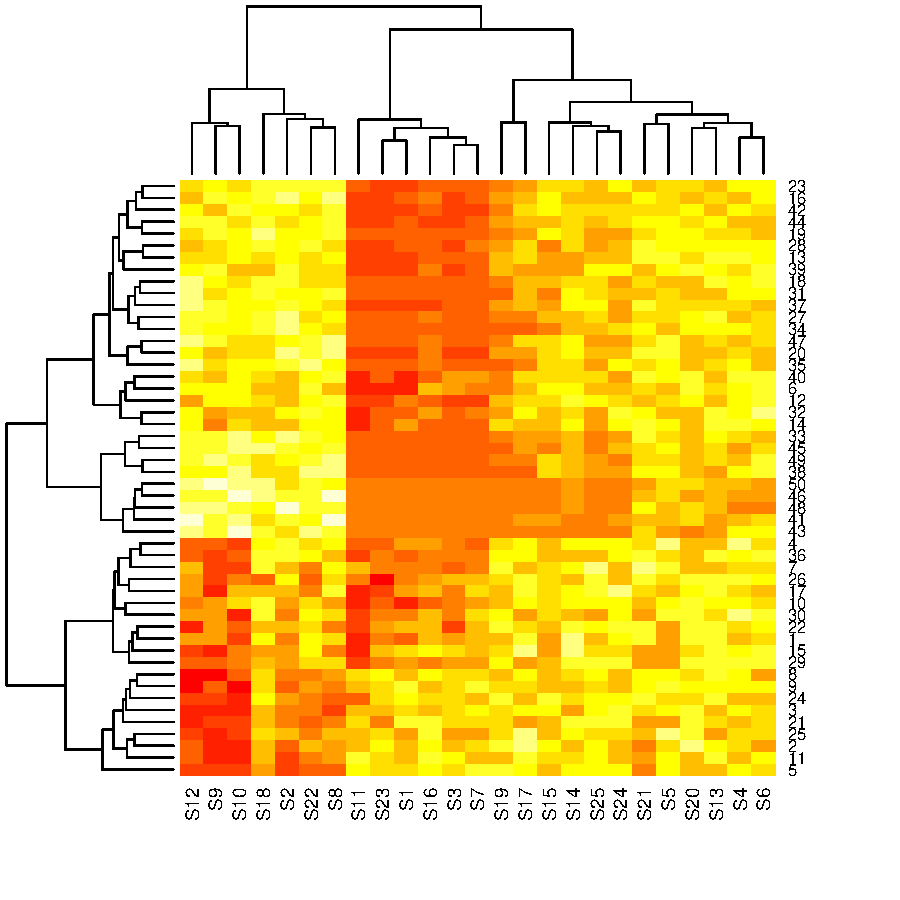
\includegraphics{ComGenR_vignette-012}

\subsection*{NMDS Ordination}

Non-metric Multidimensional Scaling (NMDS) ordination plots are a much
more common, albeit abstract means of visualizing community data. In
CG studies, it has also been used as a way to generate a trait-like
vector that can be used in quantitative genetic analyses. We can
quickly do this in \R using functions from the \textit{vegan} and
\textit{ecodist} packages:


\begin{Schunk}
\begin{Sinput}
> d <- vegdist(com)
> nms <- nmds(d,mindim=2,maxdim=2,nits=3)
\end{Sinput}
\begin{Soutput}
Using random start configuration 
Using random start configuration 
Using random start configuration 
\end{Soutput}
\begin{Sinput}
> 
\end{Sinput}
\end{Schunk}

Note here that we first calculate the Bray-Curtis dissimilarity scores
for each observation (which we call ``d''). This distance matrix in then
used to conduct the ordination. Here we set the ``mindim'' and ``maxdim''
arguments in the function to 2 so that we will get a set of
ordinations with that dimensionality. Because the NMDS procedure
starts with a randomly generated set of numbers that are then adjusted
until best represent the structure of the original distances of the
data, we have also specified the ``nits'' argument to be 3, which will
have the function output 3 ordinations. We then select the lowest
``stress'' (i.e. the best fitted) ordination from our set of three.

\begin{Schunk}
\begin{Sinput}
> nms <- nmds.min(nms)
\end{Sinput}
\begin{Soutput}
Minimum stress for given dimensionality:  0.1112529 
r^2 for minimum stress configuration:  0.9693141 
\end{Soutput}
\end{Schunk}

Note first that the fit is below the arbitrary threshold of 0.2 and
that the low number of iterations used here has been chosen purely for
example's sake. Run \texttt{?nmds} to get a more detailed description
of the NMDS and how to customize its functionality.


We can now plot our ordination, overlaying our genotype information:

\begin{Schunk}
\begin{Sinput}
> plot(nms,col=as.numeric(geno),pch=19)
> 
\end{Sinput}
\end{Schunk}
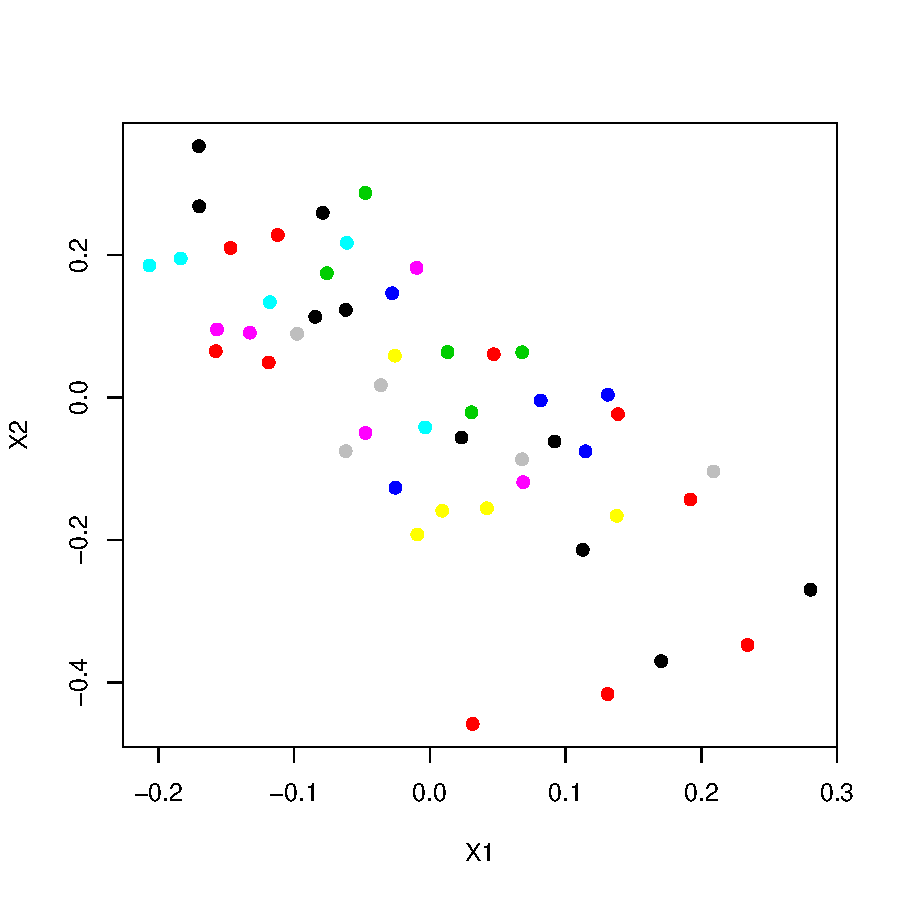
\includegraphics{ComGenR_vignette-015}

Although the stress of the ordination is low, it is still difficult to
see the patterns of the genotypes. Another method can be used to plot
our ordination using the centroids (i.e. multivariate means) and the
standard errors. This can be done easily with this function from the
\textit{ComGenR} pacakge:

\begin{Schunk}
\begin{Sinput}
> ch.plot(nms,geno,plot.legend=TRUE,loc='topright')
> 
\end{Sinput}
\end{Schunk}
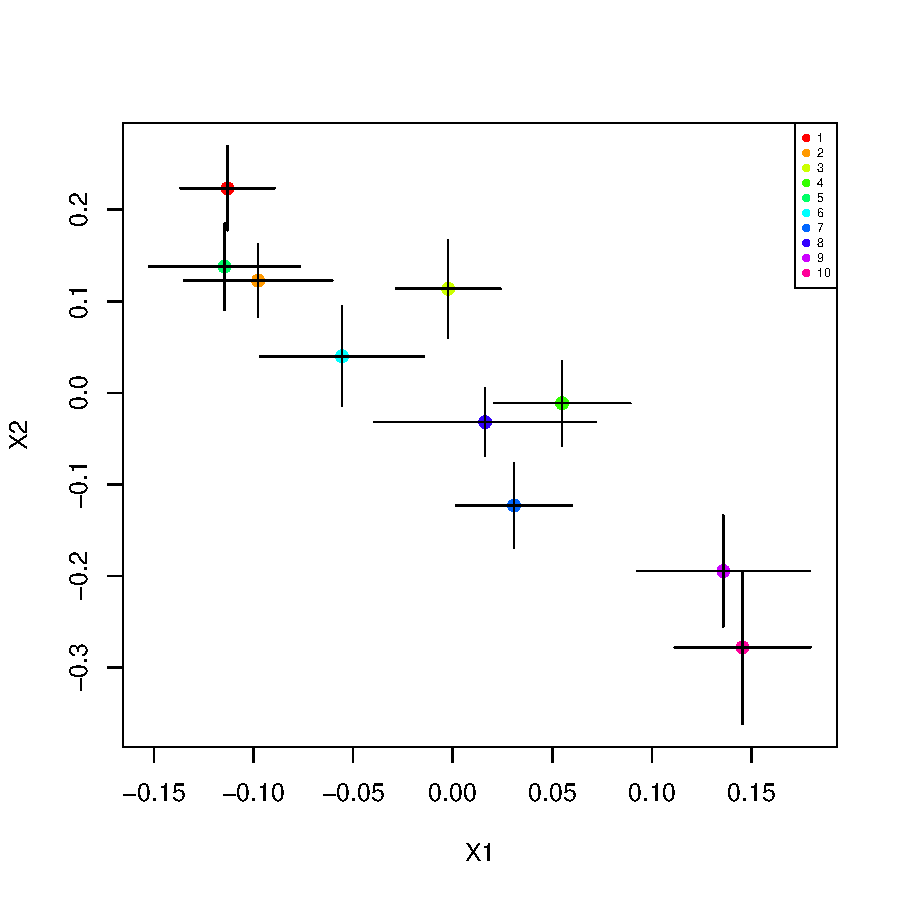
\includegraphics{ComGenR_vignette-016}

\subsection*{Vectors}

It is also easy to overlay other information (such as out phenotype) onto our ordination using
vectors:

\begin{Schunk}
\begin{Sinput}
> pheno <- the.data[,3]
> pheno.vector <- envfit(nms,pheno)
> ch.plot(nms,geno,plot.legend=TRUE,loc='topright')
> plot(pheno.vector,col='black')
> 
\end{Sinput}
\end{Schunk}
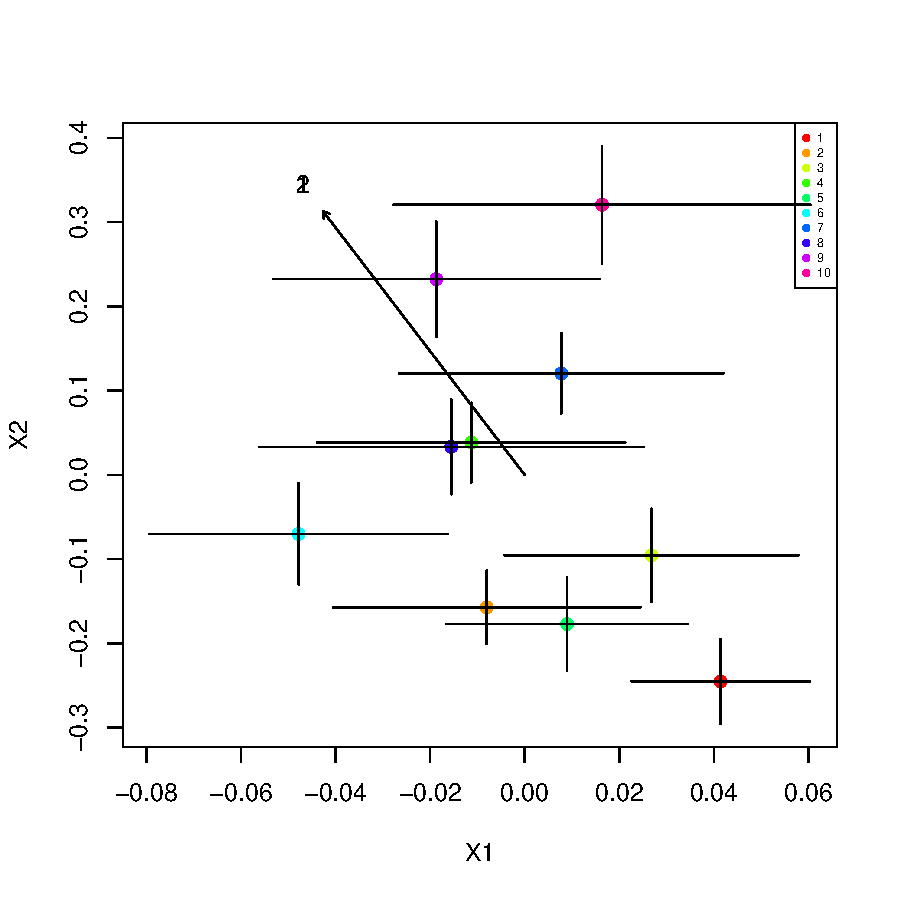
\includegraphics{ComGenR_vignette-017}


\subsection*{PerMANOVA}

%PERMANOVA - BC-distance, Clarke adjustment and adonis

Permutational Multivariate Analysis of Variance (PerMANOVA) has been
developed by ecologists, namely Marti Andersen, to address the need
for a multivariate test of compositional effects that accomodates the
often non-normal distributions of community data. We can execute it
easily in \R using the interestingly named \texttt{adonis} function
from the \textit{vegan} package:

\begin{Schunk}
\begin{Sinput}
> adonis(com~geno)
\end{Sinput}
\begin{Soutput}
Call:
adonis(formula = com ~ geno) 

Terms added sequentially (first to last)

          Df SumsOfSqs  MeanSqs F.Model      R2 Pr(>F)    
geno       9   1.44937 0.161041  6.5888 0.59718  0.001 ***
Residuals 40   0.97766 0.024442         0.40282           
Total     49   2.42703                  1.00000           
---
Signif. codes:  0 �***� 0.001 �**� 0.01 �*� 0.05 �.� 0.1 � � 1
\end{Soutput}
\begin{Sinput}
> 
\end{Sinput}
\end{Schunk}

%Pairwise PERMANOVA - p-value adjustments
The \textit{ComGenR} package provides an additional function for
conducting pairwise PerMANOVAs for levels of a single factor, such as
genotype, in order to identify the statistical differences among pairs
of levels: 

\begin{Schunk}
\begin{Sinput}
> pp.results <- pair.permanova(x=com,f=geno,nits=999)
\end{Sinput}
\begin{Soutput}
[1] "1 vs 2"
[1] "1 vs 3"
[1] "1 vs 4"
[1] "1 vs 5"
[1] "1 vs 6"
[1] "1 vs 7"
[1] "1 vs 8"
[1] "1 vs 9"
[1] "1 vs 10"
[1] "2 vs 3"
[1] "2 vs 4"
[1] "2 vs 5"
[1] "2 vs 6"
[1] "2 vs 7"
[1] "2 vs 8"
[1] "2 vs 9"
[1] "2 vs 10"
[1] "3 vs 4"
[1] "3 vs 5"
[1] "3 vs 6"
[1] "3 vs 7"
[1] "3 vs 8"
[1] "3 vs 9"
[1] "3 vs 10"
[1] "4 vs 5"
[1] "4 vs 6"
[1] "4 vs 7"
[1] "4 vs 8"
[1] "4 vs 9"
[1] "4 vs 10"
[1] "5 vs 6"
[1] "5 vs 7"
[1] "5 vs 8"
[1] "5 vs 9"
[1] "5 vs 10"
[1] "6 vs 7"
[1] "6 vs 8"
[1] "6 vs 9"
[1] "6 vs 10"
[1] "7 vs 8"
[1] "7 vs 9"
[1] "7 vs 10"
[1] "8 vs 9"
[1] "8 vs 10"
[1] "9 vs 10"
\end{Soutput}
\begin{Sinput}
> pp.results$p.mat
\end{Sinput}
\begin{Soutput}
    1     2     3     4     5     6     7     8     9    10
1  NA 0.235 0.107 0.020 0.408 0.095 0.009 0.011 0.008 0.004
2  NA    NA 0.548 0.035 0.941 0.336 0.019 0.050 0.007 0.007
3  NA    NA    NA 0.126 0.364 0.580 0.036 0.191 0.006 0.008
4  NA    NA    NA    NA 0.014 0.175 0.314 0.959 0.061 0.027
5  NA    NA    NA    NA    NA 0.188 0.017 0.035 0.009 0.009
6  NA    NA    NA    NA    NA    NA 0.047 0.324 0.022 0.015
7  NA    NA    NA    NA    NA    NA    NA 0.319 0.287 0.093
8  NA    NA    NA    NA    NA    NA    NA    NA 0.075 0.018
9  NA    NA    NA    NA    NA    NA    NA    NA    NA 0.371
10 NA    NA    NA    NA    NA    NA    NA    NA    NA    NA
\end{Soutput}
\begin{Sinput}
> 
\end{Sinput}
\end{Schunk}

Note, these p-values are not adjusted for multiple tests. It has been
stated that given the permutational nature of the test statistic used
in PerMANOVA, that this is not necessary \cite{laughlin2007}. They
can, however, be easily adjusted in \R, see the \texttt{?p.adjust}.

\subsection*{Genotype Means for Species Abundances}

Last, it is worth noting here that the \textit{ComGenR} package
contains two functions to help calculate the means and standard errors
for each species on a set of genotypes. This might be useful for
plotting:

\begin{Schunk}
\begin{Sinput}
> mean.g(com,geno)
\end{Sinput}
\begin{Soutput}
            S1        S2        S3        S4        S5        S6         S7
1  72.95872122  52.60754 76.557761 100.59891  96.87881  83.17833 85.4677456
2  56.69297651  68.53598 68.909479 103.05853 106.65108  98.44179 74.8649139
3  51.88369704  65.35430 50.616295  97.79041  92.84703 105.77472 44.1075264
4  18.25755529 109.75559 12.935158  79.39797  86.46640  82.52525 23.1239447
5  75.48528310  78.07419 62.112840  89.81027  87.05418  92.63548 70.6078202
6  44.85606705  94.02754 47.787183 107.50176  95.77763 108.14469 57.9241813
7   8.55379707 101.86531  8.110586  84.77437  70.42539  74.27427 11.8072010
8  11.38816789  96.08158 25.277710  90.53159  89.00881 100.50032 29.2444528
9   0.04378675  82.98088  0.000010  56.71628  65.07748  66.29151  0.4337885
10  0.00001000  78.97367  0.000010  31.98149  56.79711  42.79418  0.0000100
          S8        S9       S10       S11       S12       S13       S14
1   56.74694  26.39602  17.52196 65.372756  30.40270  85.22766  92.11290
2   76.10238  51.38230  57.33525 54.066535  51.98798  99.20441  96.39379
3   89.64142  55.19926  72.18741 30.189585  63.86459 105.04676  96.27458
4  108.36642  83.01691  80.04658  6.116174  89.80038  87.69209  84.81264
5   72.33276  48.19628  39.58385 53.036931  40.14465  94.32357 100.47270
6   97.64410  74.39221  72.12086 27.326698  77.13680 113.46773  89.38643
7   85.91710  82.12188  92.83378  4.033882 110.86225  83.40102  68.28648
8   99.68091  84.92606  85.77424  7.289999  88.78019  80.91477  70.95691
9  103.92340  93.30570 103.10800  0.000010 108.38613  54.35210  42.28541
10  97.17063 103.87917  90.14880  0.000010  94.49367  44.61974  38.52047
        S15       S16       S17       S18      S19       S20       S21
1  85.96763 86.019473 108.93202  79.33114 99.18178  98.19442  76.54393
2  89.30438 70.738822  91.18252  98.28993 84.72937 104.93359 100.06243
3  74.09788 56.043769  92.90926  78.58441 74.77891  85.79231  85.97045
4  83.13640 28.943160  65.06201 100.25234 43.46535  78.93218  89.84110
5  88.65563 84.227058  86.86709  94.70526 93.86222 104.96906  91.90441
6  75.73313 55.088124  77.90997 101.88877 76.73125 113.66565  93.43136
7  45.26008 17.237142  41.47292  89.36479 15.87536  67.36296  82.84907
8  64.94430 25.132405  60.66301  84.55315 50.89024  86.03285  98.27927
9  37.05411  3.200096  33.97264  94.35563 15.03518  56.38830  60.77949
10 29.06456  7.180708  18.71920  74.07238  6.84187  44.13021  49.12444
         S22       S23       S24       S25
1   66.25142 73.879707  97.72702  98.05734
2   79.29482 60.078459  88.12643 103.80586
3   88.03367 39.732162  82.25411  82.31501
4   87.78842  7.451767  69.70087  70.51218
5   76.21280 60.644732 106.01405  99.27077
6   94.14219 30.261926  85.53601  90.15915
7   98.57979  8.715062  64.58645  48.51186
8  102.14983 16.012311  68.66818  77.39797
9   84.25041  0.000010  43.63751  30.54391
10  88.80604  0.000010  11.61458  12.25931
\end{Soutput}
\begin{Sinput}
> se.g(com,geno)
\end{Sinput}
\begin{Soutput}
            S1        S2        S3        S4        S5        S6         S7
1   5.43739796 18.670058  5.778127  7.004304  8.296997  5.168865 11.3677516
2  19.33808894  6.722551  8.565175  4.272462  6.979069  7.519987 11.9702015
3  14.85762786 11.806658 19.777658  7.139296  6.754016  2.771125 14.4360210
4  13.51048754  9.275191 11.505846  4.700245  8.010242  8.925719 17.4309123
5  20.05753949 11.561569 15.598365  4.780548  9.453669  5.632065 13.0486235
6  15.03419429 12.768953 18.976293 12.665196  9.523529  8.869932 18.7127527
7   8.55378707  5.631535  8.110576  6.170892  6.561304 12.411438 11.6856331
8   9.25256856  9.351974 14.193028  9.212339  5.771482 10.184360 12.7238895
9   0.04377675 10.555517  0.000000 11.545928 16.310413  5.925743  0.4337785
10  0.00000000 10.195389  0.000000 12.029387 14.440445 19.683846  0.0000000
          S8        S9       S10       S11       S12       S13       S14
1  18.609691 15.249375  8.424058 13.287071 14.148463 10.750736 11.439359
2   8.683733 17.514793 19.384793 17.809221 18.673534  8.763967  6.320158
3  11.849952 17.252835 18.231981 21.668772 12.625390  8.041351 11.002180
4   9.498094 15.447826  4.362404  6.116164 11.243921  7.954612  5.840242
5  13.046998 16.228164 13.450362 14.667054 12.644679  9.981228  6.680258
6   4.536860 11.555202 13.455153 14.193351 11.551900  5.057715 11.138096
7   4.748334  8.108177  7.069453  4.033872  4.971996  9.002124  8.033439
8   9.447377 15.950437 12.165406  7.289989 12.373326 13.305234  7.910734
9   7.501465  8.958307  6.514739  0.000000  5.783432 15.259269 17.668598
10 11.834437  8.767616  6.566103  0.000000 10.114481 12.524265 16.201040
         S15       S16       S17       S18       S19       S20       S21
1   7.567003  6.629286  5.001266 12.483897  6.514305 11.018625 13.626689
2   5.600815  9.237984  6.976859  8.835930 11.191024  8.131273  6.682346
3   6.179000 20.450765 10.425164  3.726023  5.034212  6.581304 11.988811
4   6.466336 13.869177 12.057774 10.412588 11.321905  7.884235  8.444292
5   7.532464 14.975124 12.326897  9.743686 14.279270  5.397849 11.091566
6  12.603375 13.509516 14.671140 12.167747 18.913283  6.094358 10.780627
7  11.476068 11.137053 15.463569  6.814927 11.635601  8.256831  8.762707
8   7.156257 11.114869 17.465461  7.163573 16.764906 12.798263  9.994269
9  18.900828  3.200086 15.159717 13.846307  9.321271 14.583797 11.159802
10 18.218019  7.180698 14.681206  7.146889  4.642727  8.403332 13.257250
         S22       S23       S24       S25
1  16.328481 10.582029  7.176362  3.207189
2  11.490827 17.974677  7.989786  7.243416
3   9.118039 18.468054  5.600795  9.194714
4   9.074147  7.451757 13.733018 10.588776
5  16.334576 16.471093  4.914319  8.206593
6   8.624746 12.923827 15.426250 12.377842
7   7.541532  8.715052 12.525196 10.288491
8   5.467973 10.587743 13.575491 12.240856
9   6.151666  0.000000 14.992092 17.653522
10  8.582013  0.000000  8.876805  7.967191
\end{Soutput}
\begin{Sinput}
> 
\end{Sinput}
\end{Schunk}

\section{Modeling and Quantifying Heritability}

Community Genetics also seeks to quantify how much variation in the
community is explained by genetic variation. The \textit{ComGenR}
package has several functions for both modeling and quantifying the
community level effects of genetic variation as developed in the
Shuster et al. 2006 \cite{shuster2006} article. 

\subsection*{Simulating Community Genetics}
%cgSIM - genetic versus environmental variance

In general, simulation modeling is a useful tool for exploring
possible mechanistic explainations for patterns. As community
geneticists are interested in understanding how genetics influences
community patterns, it is useful to have a simple simulation
framework. \textit{ComGenR} provides a set of functions to do
this. Described more fully here \cite{shuster2006}, briefly the model
simulates the response of a community of dependent species to
selection imposed by genetically based phenotypic variation in a
foundation species. This can be done by first creating a set of
``trees'' and a set of ``insects'' that form a dependent community. This
can be done by hand, but \textit{ComGenR} provides two functions to
easily do this:

\begin{Schunk}
\begin{Sinput}
> trees <- gpmTrees()
> insects <- gpmCom()
> 
\end{Sinput}
\end{Schunk}

Note the structure of these two matrices:

\begin{Schunk}
\begin{Sinput}
> head(trees)
\end{Sinput}
\begin{Soutput}
     geno pheno
[1,]    1  11.0
[2,]    1  11.0
[3,]    1  11.0
[4,]    1  11.0
[5,]    1  11.0
[6,]    2  12.5
\end{Soutput}
\begin{Sinput}
> head(insects)
\end{Sinput}
\begin{Soutput}
         [,1]      [,2]
[1,] 4.582360  5.510218
[2,] 4.528272  6.018267
[3,] 5.347606  6.571729
[4,] 7.952068  9.428625
[5,] 9.800800 10.104148
[6,] 8.240022  9.000200
\end{Soutput}
\end{Schunk}

The ``trees'' matrix has two columns: geno and pheno. The ``geno'' value is the
genotype of each tree in each row and ``pheno'' is the associated
phenotype that is used to determine the effect of that tree on the
arthropod community. The ``insects'' matrix has phenotypic values for
each insect species in each row. These ``insect'' values are generated
randomly using a heterkaryotic genome model from within a range of
user determined values for each of two alleles. 

Now, these values can be used to simulate the response of a community
of arthropods:

\begin{Schunk}
\begin{Sinput}
> our.sim <- cgSim(trees,insects,reps=1,YY=5,GG=5)
\end{Sinput}
\begin{Soutput}
[1] "1 1 1"
[1] "1 1 2"
[1] "1 1 3"
[1] "1 1 4"
[1] "1 1 5"
[1] "1 2 1"
[1] "1 2 2"
[1] "1 2 3"
[1] "1 2 4"
[1] "1 2 5"
[1] "1 3 1"
[1] "1 3 2"
[1] "1 3 3"
[1] "1 3 4"
[1] "1 3 5"
[1] "1 4 1"
[1] "1 4 2"
[1] "1 4 3"
[1] "1 4 4"
[1] "1 4 5"
[1] "1 5 1"
[1] "1 5 2"
[1] "1 5 3"
[1] "1 5 4"
[1] "1 5 5"
\end{Soutput}
\begin{Sinput}
> 
\end{Sinput}
\end{Schunk}

This outputs a set of simulated communities. The ``reps'', ``YY'' and ``GG'' arguments
determine the number of iterations, environmental scenarios and
selection intensity scenarios. For each environmental scenario the
effect of the genetic variance is heald constant and the amount of
random noise introduced by non-genetic influences is
increased. Similarly, each selection intensity scenario increases the
effect of genetic variation while holding the influence of the
environment constant. 

%Isolating an NMDS axis - pros-cons and possible pitfalls
\subsection*{NMDS Community Trait}

Per the methods of Shuster et al. 2006, we can take one of our
simulated matrices and summarize the variation of the community with
an NMDS ordination. This is done in order to be able to treat the
multivariate community as a univariate trait that has similar
statistical properties as traits analyzed in quantitative genetics
(e.g. univariate and normally distributed). We can use the same
ordination methods that we used above to get a single NMDS ordination
axis for a simulated community:

\begin{Schunk}
\begin{Sinput}
> com.sim <- our.sim[[1]][[1]][[5]]
> d <- vegdist(com.sim)
> nms.sim <- nmds(d,mindim=1,maxdim=1)
\end{Sinput}
\begin{Soutput}
Using random start configuration 
Using random start configuration 
Using random start configuration 
Using random start configuration 
Using random start configuration 
Using random start configuration 
Using random start configuration 
Using random start configuration 
Using random start configuration 
Using random start configuration 
\end{Soutput}
\begin{Sinput}
> nms.sim <- nmds.min(nms.sim)
\end{Sinput}
\begin{Soutput}
Minimum stress for given dimensionality:  0.223228 
r^2 for minimum stress configuration:  0.8989635 
\end{Soutput}
\begin{Sinput}
> nms.sim <- nms.sim[,1]
> 
\end{Sinput}
\end{Schunk}

\begin{Schunk}
\begin{Sinput}
> hist(nms.sim)
\end{Sinput}
\end{Schunk}
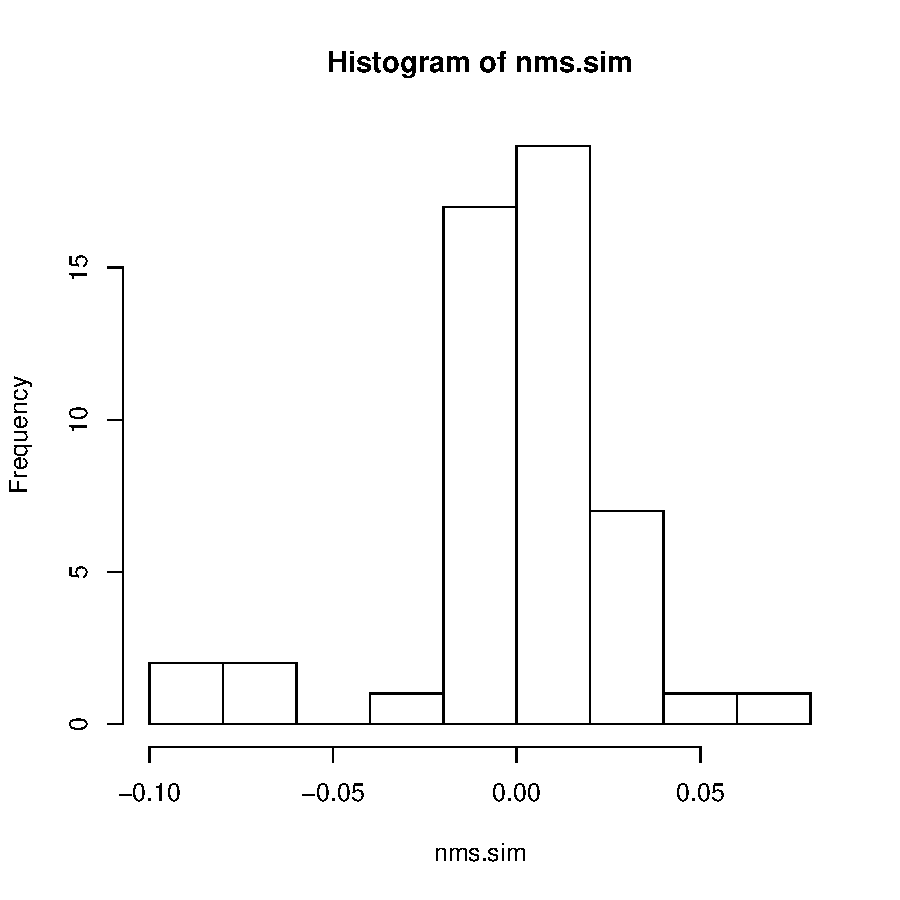
\includegraphics{ComGenR_vignette-025}

In this output, note both the stress and the $r^2$ of the final
configuration. This similarly indicates how well the ordination
represents the original data. As one would expect, this representation
is never perfect as it is intended to be an abstraction of the
original data. The user should be familiar with the meaning of
ordinated scores and how they can and should be interpreted. 


\subsection*{Community Heritability}
%getH2C - balanced and unbalanced design auto-detect
We can now use this ordinated representation of the community to
calculate the community heritability value for this simulated
population of trees:

\begin{Schunk}
\begin{Sinput}
> geno.sim <- factor(trees[,1])
> getH2C(nms.sim,geno.sim)
\end{Sinput}
\begin{Soutput}
      H2C        CI        SE 
0.4567207 0.3172969 0.1618862 
 lower.CI       H2C  upper.CI 
0.1394239 0.4567207 0.7740176 
\end{Soutput}
\begin{Sinput}
> 
\end{Sinput}
\end{Schunk}

The output gives heritability score for the community, as represented
by the ordination, along with associated confidence limits. 

\section{Network Modeling and Co-occurrence Analyses}

Community Ecology and Community Genetics deal with complex sets of
organisms largely because these fields aknowledge the need to study
groups of organisms. A primary motivation for this is that species
interact and these interactions contribute to variation in their
distributions, abundances and function. Thus, communities are formed
by webs or networks of interacting species and a complete
understanding of communities requires an understanding of these
networks. Thus, the \textit{ComGenR} package provides tools for both
modeling and analyzing relationships among species comprising
communities. 

%What do co-occurrences tell us?

\subsection*{Null-Model Co-occurrence Analysis}

Given the motivation described above, it is unfortunate that
interaction data is exceedingly rare and difficult to obtain for
ecological studies. Initially developed for biogrogrphic studies,
co-occurrence analysis was developed to bridge this information
gap. At its inception \cite{diamond1975}, the analysis of species
co-occurrence patterns was inteded to generate and test hypotheses
about how communities assemble \cite{gotelli2000}. It was posited that
interactions among species influenced the distribution of species in
space, namely through competitive exclusion \cite{diamond1975}, though
later work has demonstrated the importance of positive interactions
\cite{maestre2009}. 

Analyzing co-occurrence patterns in CG data provides a well developed
means to examine the co-variances among species. Once the effect of
genetic variation on community composition has been established,
co-occurrence analysis can then be used to examine the overarching
structure in the commuity data due in part to that genetic effect. To
do this, we use permutation based null modeling tools provided in the
\textit{vegan} package. \textit{ComGenR} provides high level access to
these functions, so that these analyses can be performed as follows:

%Co-occurrence (overall)

\begin{Schunk}
\begin{Sinput}
> com[com<1] <- 0
> cnm.test(com,nits=25)
\end{Sinput}
\begin{Soutput}
  |                                                        
  |                                                  |   0%
  |                                                        
  |++                                                |   4%
  |                                                        
  |++++                                              |   8%
  |                                                        
  |++++++                                            |  12%
  |                                                        
  |++++++++                                          |  16%
  |                                                        
  |++++++++++                                        |  20%
  |                                                        
  |++++++++++++                                      |  24%
  |                                                        
  |++++++++++++++                                    |  28%
  |                                                        
  |++++++++++++++++                                  |  32%
  |                                                        
  |++++++++++++++++++                                |  36%
  |                                                        
  |++++++++++++++++++++                              |  40%
  |                                                        
  |++++++++++++++++++++++                            |  44%
  |                                                        
  |++++++++++++++++++++++++                          |  48%
  |                                                        
  |++++++++++++++++++++++++++                        |  52%
  |                                                        
  |++++++++++++++++++++++++++++                      |  56%
  |                                                        
  |++++++++++++++++++++++++++++++                    |  60%
  |                                                        
  |++++++++++++++++++++++++++++++++                  |  64%
  |                                                        
  |++++++++++++++++++++++++++++++++++                |  68%
  |                                                        
  |++++++++++++++++++++++++++++++++++++              |  72%
  |                                                        
  |++++++++++++++++++++++++++++++++++++++            |  76%
  |                                                        
  |++++++++++++++++++++++++++++++++++++++++          |  80%
  |                                                        
  |++++++++++++++++++++++++++++++++++++++++++        |  84%
  |                                                        
  |++++++++++++++++++++++++++++++++++++++++++++      |  88%
  |                                                        
  |++++++++++++++++++++++++++++++++++++++++++++++    |  92%
  |                                                        
  |++++++++++++++++++++++++++++++++++++++++++++++++  |  96%
  |                                                        
  |++++++++++++++++++++++++++++++++++++++++++++++++++| 100%
      SES   lower.p   upper.p 
-31.73185   0.00000   1.00000 
\end{Soutput}
\begin{Sinput}
> 
\end{Sinput}
\end{Schunk}

It is important to consider a threshold of detection for species prior
to running co-occurrence analysis, since it does not use abundance
data but presence-absence data (i.e. occurrences and non-occurrences).
Here, we set values less than 1 to zero.

%Network (overall)

Although co-occurrence analyses allow us to test for the average
structure of co-occurrence patterns in the community, they do not
resolve the structure those patterns. Although the network approach
has been employed in ecology for a relatively long time
(e.g. \cite{macarthur1955}), recent developments in analytical methods
have expanded utility and scope of this approach
\cite{araujo2011}. The \textit{ComGenR} package provides several
functions for the user to analyze CG data using a network modeling and
analytical approach. 

First to compliment the co-occurrence analysis, it is extremely useful
to plot community data as a bipartite network. This re-representation
of the data in this context allows for the examination of
co-occurrence patterns. To do this, we use tools from the
\textit{bipartite} package:


\begin{Schunk}
\begin{Sinput}
> com. <- com
> com.[com.<=85] <- 0 
> com. <- com.[,order(apply(com,2,sum),decreasing=TRUE)]
> rownames(com.) <- the.data$tree.id
> geno.color <- rainbow(nlevels(geno))[as.numeric(geno)]
> plotweb(com.,method='normal',col.low=geno.color,text.rot=90)
> 
\end{Sinput}
\end{Schunk}

It's useful to note here that previous studies of bipartite networks
in ecology have shown that these networks tend to have a nested
structure that has potentially stabilizing effects on the community as
a whole \cite{bascompte2003}. The \textit{bipartite} package provides
a means to test for this. For more information see \texttt{?nestedness}.


%%%NOTE: Araujo links co-occurrence and compositional analyses through
%%%the use of distances/dissimilarities

Next, we can use another network approach to examine these
co-occurrence patterns with regard to the relationship \textit{among}
species in the community matrix. Before do so, it is important to
provide a brief caveat. This approach is meant to explore the data,
and, toward this end, it provides a perspective that appears to
resolve interactions among species. While this may be the case, this
is not testable with the analysis itself. It is up to the user to
decide to what extent these results can be used to speak to the
structure of true ecological interactions (e.g. trophic or
pollination) given the nature of the data and other information about
the community. However, analysis is only useful with appropriate
interpretation, and it can be argued that ecological interactions tend
to occur locally, and, thus if species are observed at an appropriate
scale, it is possible to make inferences about the potential for
interactions to occur, given non-random patterns of co-occurrence
\cite{araujo2011}.

Here is how to conduct the co-occurrence based network modeling
described in Araujo et al. 2011 \cite{araujo2011} in the
\textit{ComGenR} package:


%% <<fig=true>>=
%% net <- CoNetwork(com.)
%% net
%% @ 

Once this network has been generated, we can now
plot. \textit{ComGenR} provides an easy to use function built on the
\texttt{gplot} function in the \textit{sna} package:

\begin{Schunk}
\begin{Sinput}
> mgp(net,com.,displaylabels=TRUE)
\end{Sinput}
\begin{Soutput}
              x          y
 [1,]  5.614751  -9.535275
 [2,]  1.338922 -11.474190
 [3,] 16.116442 -20.362397
 [4,] -3.451333 -22.920559
 [5,] -3.065037 -16.522574
 [6,] -1.116131 -13.951938
 [7,]  1.960119 -30.753059
 [8,] 12.551329 -27.912783
 [9,] -3.331103 -19.505581
[10,] -2.204218 -27.081051
[11,]  9.029850 -29.315938
[12,]  7.619237 -24.238016
[13,]  4.540129 -20.692295
[14,]  9.661871 -24.103821
[15,]  5.471840 -19.711264
[16,]  5.847568 -24.772816
[17,]  8.440877 -23.109704
[18,] 11.449649 -10.475973
[19,]  5.304449 -22.437530
[20,]  9.605370 -20.498507
[21,]  7.893931 -18.248979
[22,] 12.689082 -20.131207
[23,] 13.643471 -18.158497
[24,] 12.498651 -21.559228
[25,] 11.579958 -17.268726
\end{Soutput}
\end{Schunk}
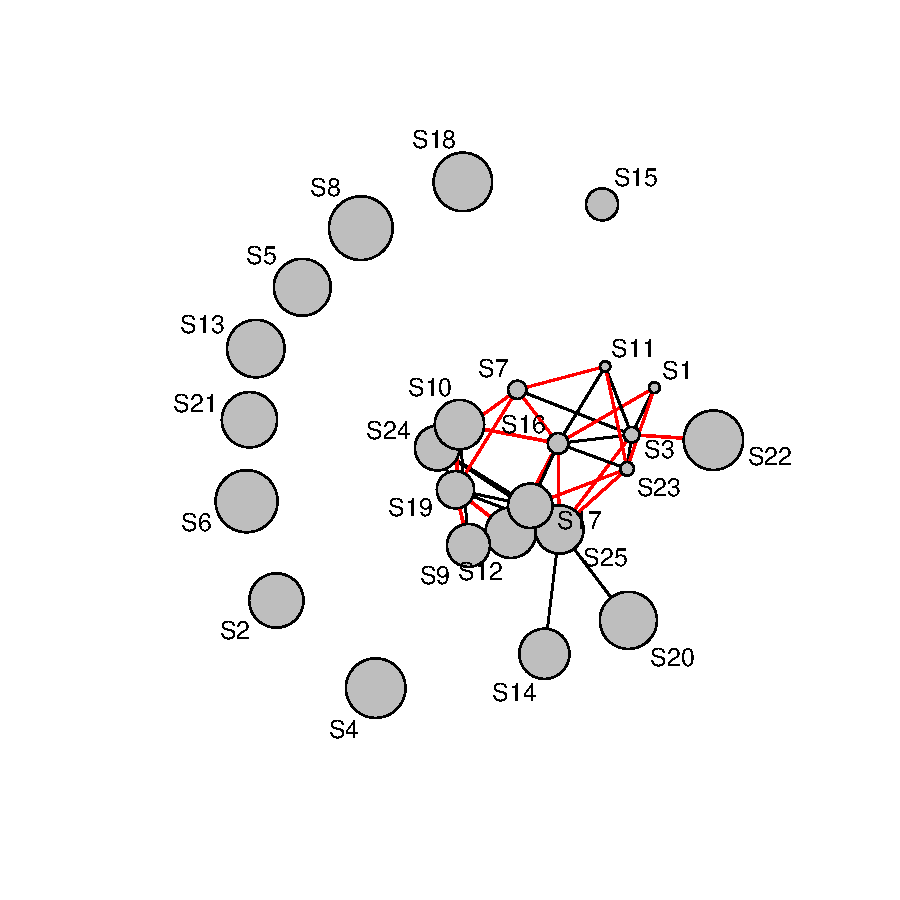
\includegraphics{ComGenR_vignette-029}


\section{A Template Analysis}

%PERMANOVA - genotype
%Paired PERMANOVA
%NMDS - with overlays
%Calculate heritability
%Co-occurrence analysis (R1)
%Network model (stand - all and condensed)
%Tree level co-occurrence (genotype effect test)
%Tree level network (average)

To help guide the user, we present a template for using the package
and how one might go about conducting an analysis on a dataset from a
CG study.

\begin{Schunk}
\begin{Sinput}
> library(ComGenR)
>                                         #model community data
> trees <- gpmTrees()
> com.sim <- cgSim(tree.pheno=trees,reps=1,YY=5,GG=7)
> com <- com.sim[[1]][[5]][[7]]
> geno <- factor(trees[,1])
>                                         #composition
> adonis(com~geno)
> nms <- nmds(vegdist(com),2,2,nits=3)
> my.nms <- nmds.min(nms)
> ch.plot(my.nms,g=geno,plot.legend=FALSE)
> top.ten <- com[,order(apply(com,2,sum),decreasing=TRUE)][,1:10]
> plot(envfit(my.nms,top.ten),add=TRUE,col='darkgrey')
>                                         #heritability
> getH2C(com,geno)
>                                         #networks
> net <- CoNetwork(com,threshold=20)
> mgp(net,com,displaylabels=TRUE)
> mgp(min.net(net,com)[[1]],min.net(net,com)[[2]],displaylabels=TRUE)
>                                         #co-occurrence
> cnm.results <- cnm.test(com,nits=100,threshold=10)
> cnm.results
> 
> 
\end{Sinput}
\end{Schunk}



%% %%Figure construction
%% <<echo=false,results=hide,label=fig1,include=false>>=
%% @ 

%% %%Figure plotting
%% \begin{figure} 
%% \begin{center} 
%% <<label=fig1,fig=TRUE,echo=false>>=
%% <<fig1>> 
%% @ 
%% \end{center} 
%% \caption{}
%% \label{fig:one}
%% \end{figure}


%% %%Activate for bibtex vibliography
\bibliographystyle{unsrt}
\bibliography{ComGenR_vignette.bib}


\end{document}  


